%auto-ignore
\section{Introduction}

% \vspace{-40pt}
% \begin{align}
% \center \hspace{40pt}
% \parbox{.45\columnwidth}{\raggedright\textit{``O for a Muse of fire, that would ascend \\
% The brightest heaven of invention''} \\
% \raggedleft\textemdash{} William Shakespeare, Henry V}
% \vspace{-30pt}
% \end{align}

Generative image models conditioned on text prompts have taken an enormous leap in quality and flexibility in the last few years \citep{dalle2,glide,imagen,parti,ldm,midjourney}. This was enabled by a combination of deep learning architecture innovations \citep{vqvae,vaswani2017attention}; novel training paradigms such as masked modeling for both language \citep{bert,t5xxl} and vision tasks \citep{MAE,maskgit}; new families of generative models such as diffusion \citep{ddpm,ldm,imagen} and masking-based generation \citep{maskgit}; and finally, the availability of large scale image-text paired datasets \citep{laion}. 

\newcommand{\figwidth}{1.0\textwidth}

\begin{figure*}[ht!]
\vspace{-15pt}
\centering
\captionsetup{width=\figwidth}
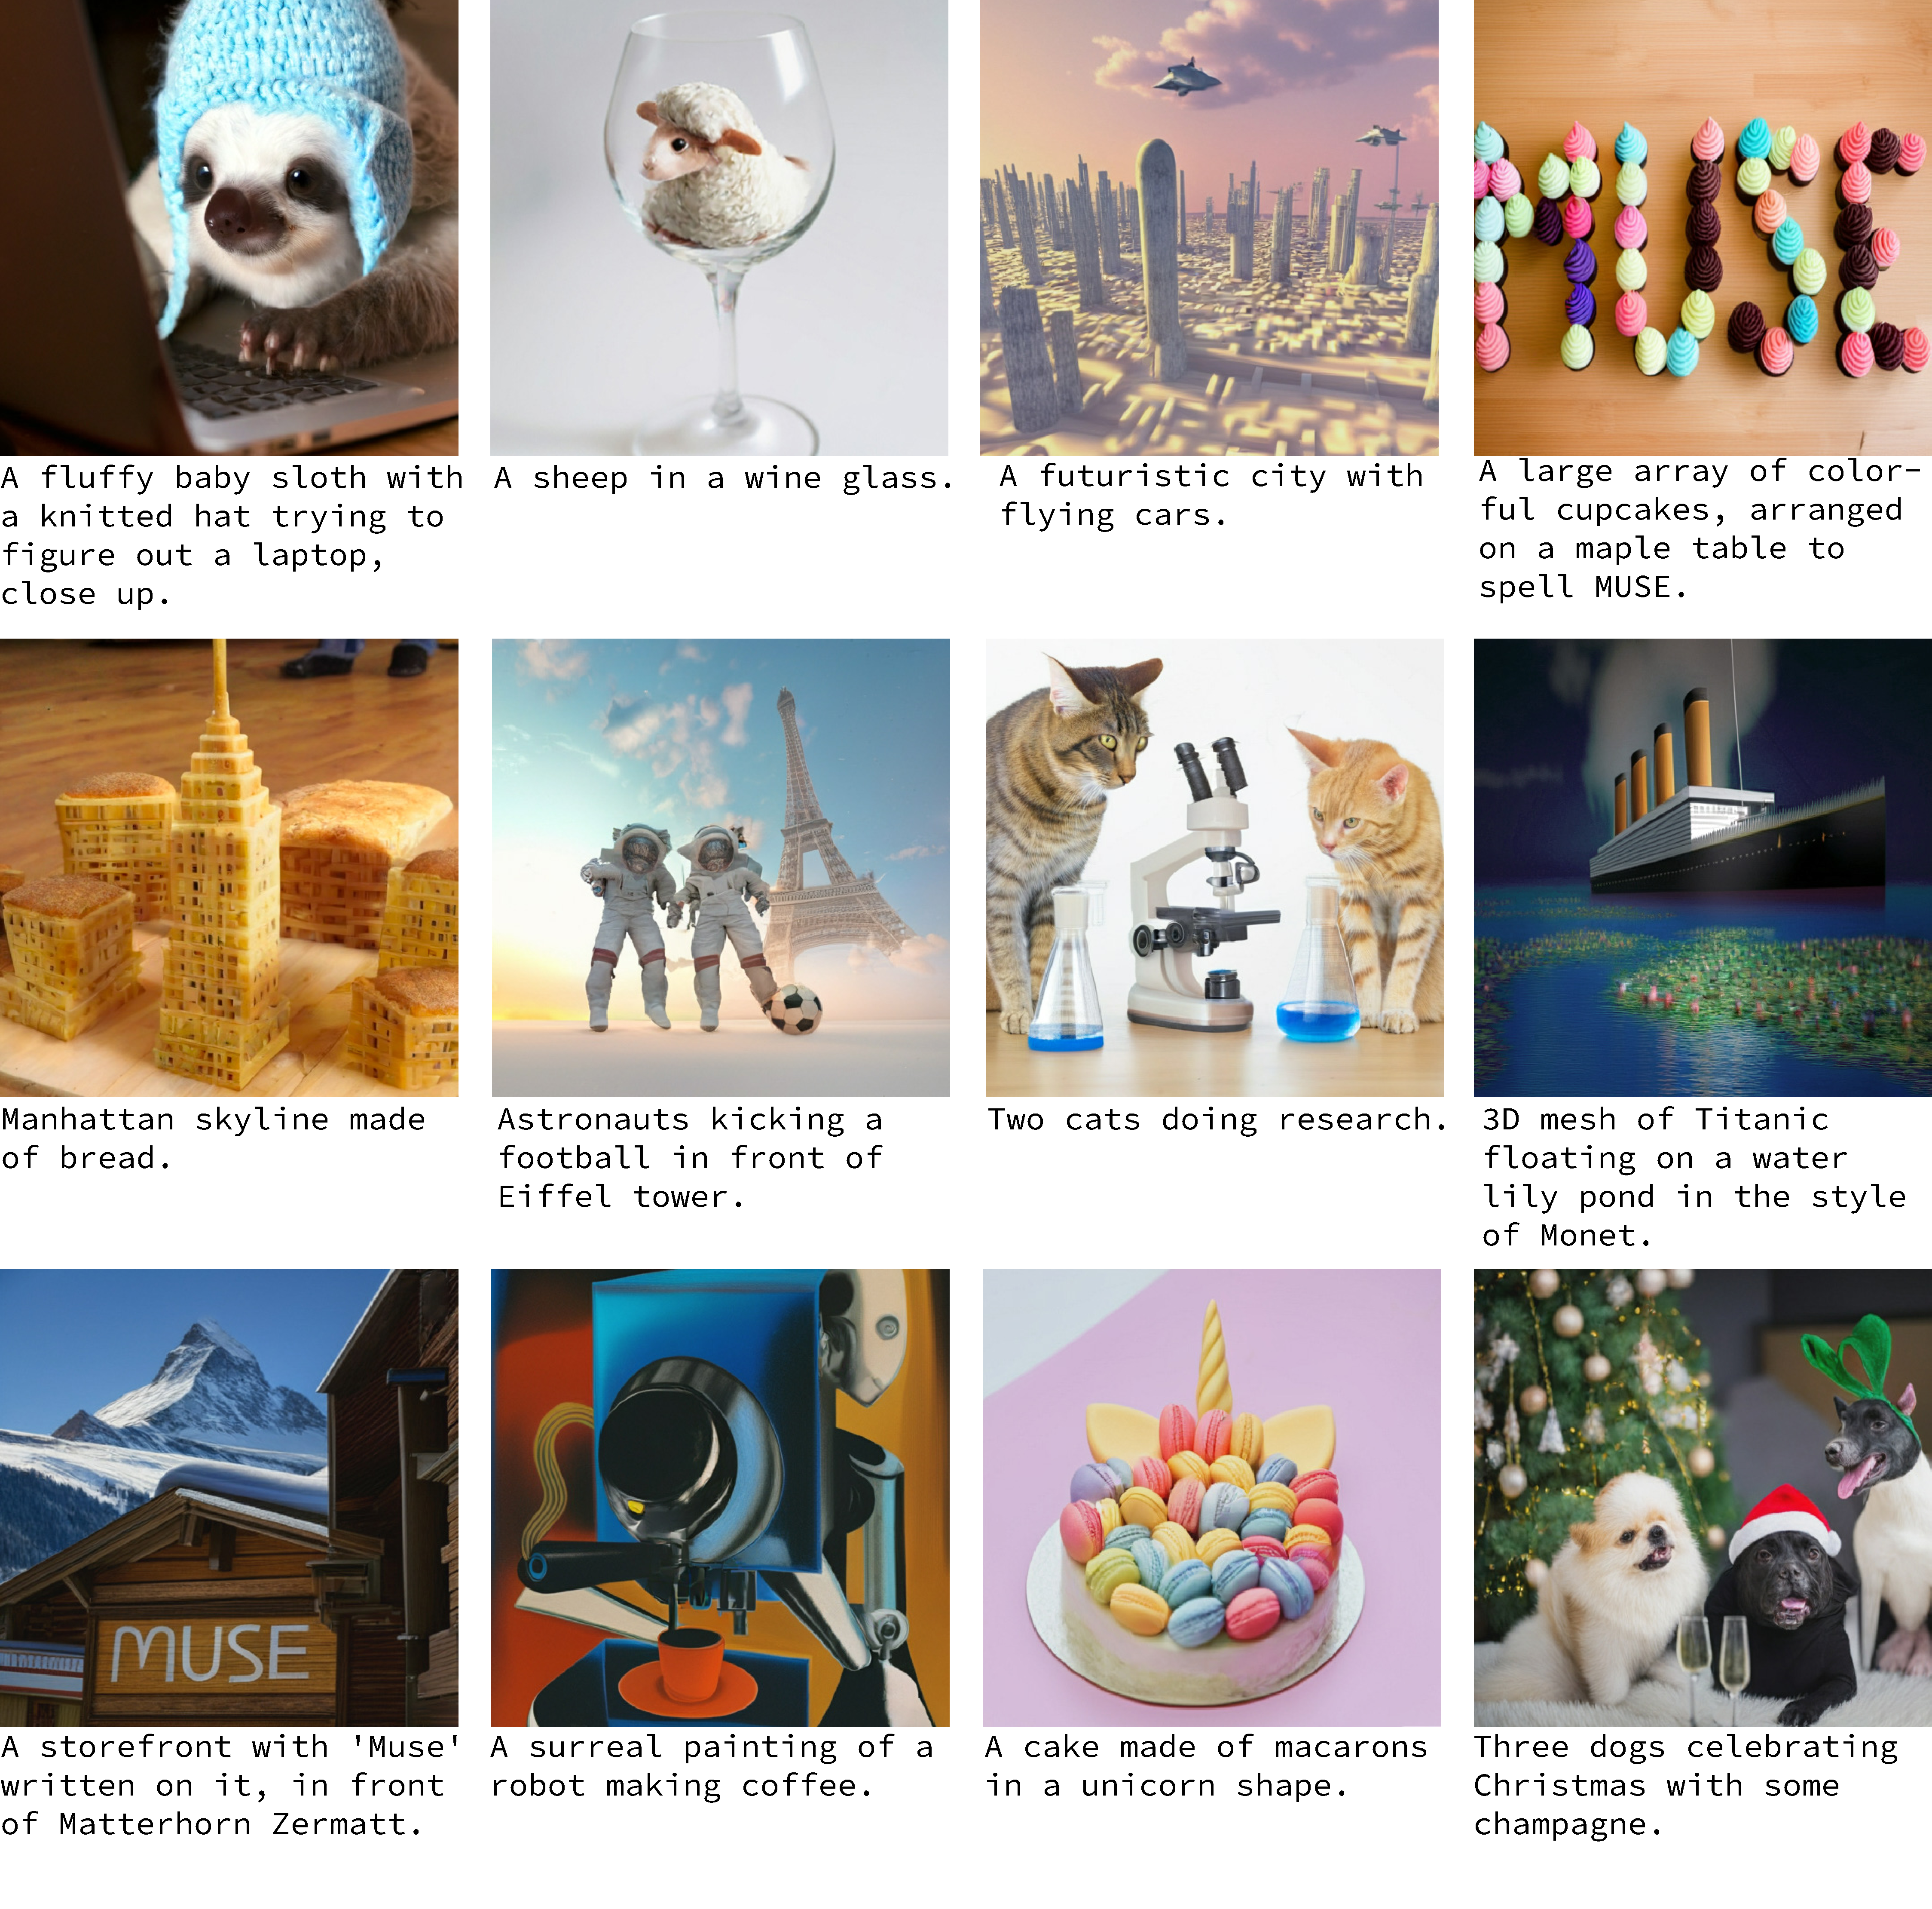
\includegraphics[width=\figwidth]{figs/teaser_v1}
% huiwen: trying to find some good substitutes
\vspace{-23pt}
\caption{\small \name~text-to-image generation ($512 \times 512$ resolution). Under each generated image, the corresponding caption is shown, exhibiting a variety of styles, captions and understanding. Each image was generated in $1.3$s on a TPUv4 chip. 
% \aj{Nit: Top middle prompt: Salvador Dali ends in an unmatched quotation.}
%Further examples are given elsewhere in the paper and at \url{\website}.
}
\label{fig:teaser_t2i}
\end{figure*}

\renewcommand{\figwidth}{1.0\textwidth}
\begin{figure*}[ht!]
% \vspace{-10pt}
\centering
\captionsetup{width=\figwidth}
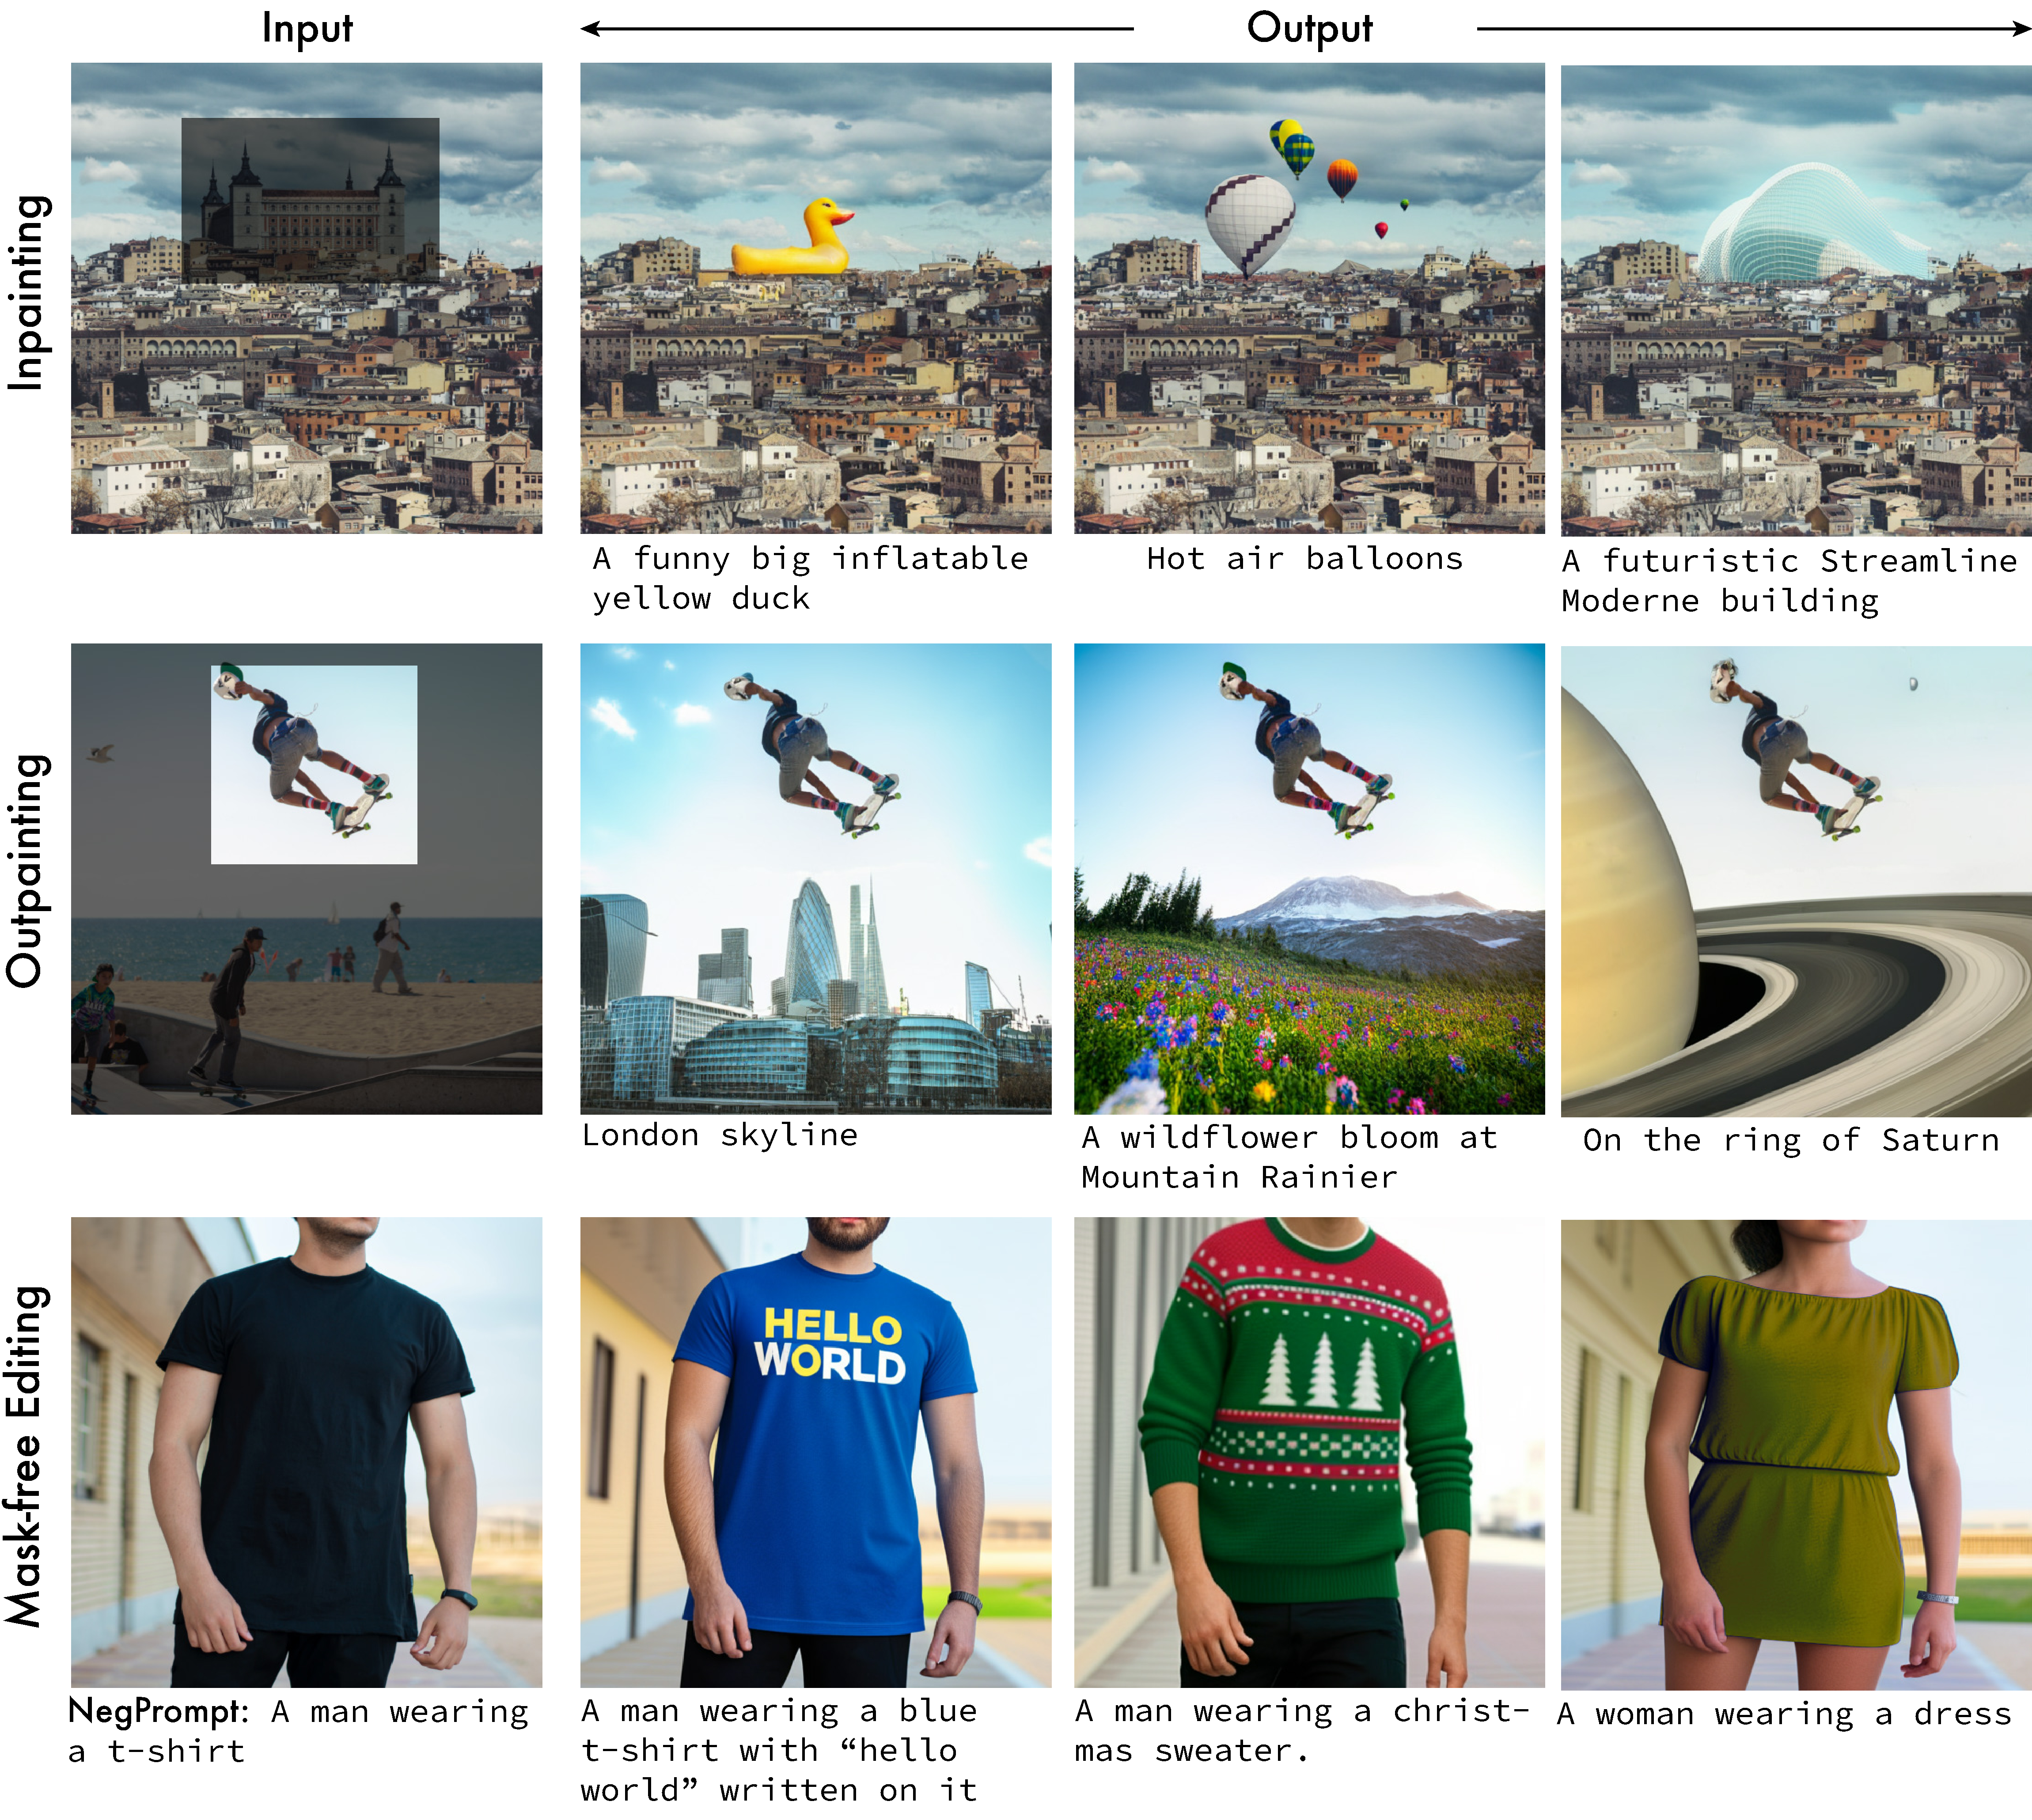
\includegraphics[width=\figwidth]{figs/teaser_editing_1}
\vspace{-18pt}
\caption{\small Examples of zero-shot text-guided image editing using \name. We show examples of a number of editing applications using the \name ~text-to-image generative model, on \emph{real} input images, without fine-tuning. All edited images are generated at $512\times512$ resolution. % \aj{``Text-guided extrapolation'' is referred to as ``Text-guided outpainting'' everywhere else in the paper.}
%Further examples are given elsewhere in the paper and at \url{\website}.
}
\vspace{-5pt}
\label{fig:teaser_edit}
\end{figure*}


In this work, we present a new model for text-to-image synthesis using a masked image modeling approach \citep{maskgit}. Our image decoder architecture is conditioned on embeddings from a pre-trained and frozen T5-XXL \citep{t5xxl} large language model (LLM) encoder. In agreement with Imagen \citep{imagen}, we find that conditioning on a pre-trained LLM is crucial for photorealistic, high quality image generation. Our models (except for the VQGAN quantizer) are built on the Transformer \citep{vaswani2017attention} architecture. 
%\jarred{replace this sentence based on new name} 
% We name our text-to-image generation model \name~after the great Polymath Leonardo DaVinci \citep{davinciwiki}, who was skilled at painting, draughting and sculpting. \aj{Need to update this sentence.}

We have trained a sequence of \name~models, ranging in size from 632M parameters to 3B parameters (for the image decoder; the T5-XXL model has an additional 4.6B parameters). Each model consists of several sub-models (\figg{model}):
First, we have a pair of VQGAN ``tokenizer'' models \citep{esser2021taming}, which can encode an input image to a sequence of discrete tokens as well as decode a token sequence back to an image. We use two VQGANs, one for 256x256 resolution (``low-res'') and another for 512x512 resolution (``high-res''). Second, we have a base masked image model, which contains the bulk of our parameters. This model takes a sequence of partially masked low-res tokens and predicts the marginal distribution for each masked token, conditioned on the unmasked tokens and a T5XXL text embedding. Third, we have a ``superres'' transformer model which translates (unmasked) low-res tokens into high-res tokens, again conditioned on T5-XXL text embeddings. We explain our pipeline in detail in \secc{model}.

% The first is a VQGAN vector quantization model \citep{esser2021taming}, where the encoder converts an input image into a sequence of quantized tokens. This set of tokens is then masked so that a certain (variable) fraction of them is passed into the second model, along with the output embedding from a T5-XXL model from a given image-text caption pair in the dataset. The text embedding is used with cross-attention to image tokens. Similar to MaskGIT \citep{maskgit}, the model is trained to predict discrete quantized tokens. The final predicted tokens are passed to the third model which super-resolves the output to a finer-grained latent space, followed by decoding to a higher final spatial resolution ($512 \times 512$), which is based on a second VQGAN model. We also deploy classifier-free guidance \citep{ho2022classifier} to further increase quality of the generated outputs for both the base and super-resolution models. Our pipeline is explained in detail in \secc{model} and shown in \figg{model}. \dilip{Pls verify details in this paragraph}

Compared to Imagen \citep{imagen} or Dall-E2 \citep{dalle2} which are built on cascaded pixel-space diffusion models, \name~is significantly more efficient due to the use of discrete tokens; it can be thought of as a discrete diffusion process with the absorbing state (\mask)~\citep{austin2021structured}. Compared to Parti \citep{parti}, a state-of-the-art autoregressive model, \name~is more efficient due to the use of parallel decoding.
Based on comparisons on similar hardware (TPU-v4 chips), we estimate that \name~is more than $10$x faster at inference time than either Imagen-3B or Parti-3B models and $3$x faster than Stable Diffusion v1.4 \citep{ldm} (see \secc{speed}). All these comparisons are when images of the same size: either $256\times256$ or $512\times512$. \name~is also faster than Stable Diffusion \citep{ldm}, in spite of both models working in the latent space of a VQGAN. We believe that this is due to the use of a diffusion model in Stable Diffusion v1.4 which requires a significantly higher number of iterations at inference time.

The efficiency improvement of \name, however, does \emph{not} come at a loss of generated image quality or semantic understanding of the input text prompt. We evaluate our output on multiple criteria, including CLIP score \citep{clip} and FID \citep{fid}. The former is a measure of image-text correspondence; and the latter a measure of image quality and diversity. Our 3B parameter model achieves a CLIP score of \cococlip~and an FID score of \cocofid~on the COCO \citep{coco} zero-shot validation benchmark, which compares favorably with that of other large-scale text-to-image models (see \tabb{eval_coco}). %Our 632M parameter model achieves a state of the art FID score of \ccfidbase~ 
Our 632M(base)+268M(super-res) parameter model achieves a state of the art FID score of \ccfidsr~ when trained and evaluated on the CC3M \citep{sharma2018conceptual} dataset, which is significantly lower than all other reported results in the literature (see \tabb{eval_cc3m}). We also evaluate our generations on the PartiPrompts \citep{parti} evaluation suite with human raters, who find that \name~generates images better aligned with its text prompt $2.7$x more often than Stable Diffusion v1.4 \citep{ldm}. 
%\dilip{AJ to fill details and add a figure in Results section and point to it here}.

\name~generates images that reflect different parts of speech in input captions, including nouns, verbs and adjectives.
%Furthermore, there is evidence of properties such as compositionality and cardinality. Different image styles are captured.
Furthermore, we present evidence of multi-object properties understanding, such as compositionality and cardinality, as well image style understanding.
See \figg{teaser_t2i} for a number of these examples and our website \url{http://\website} for more examples. The mask-based training of \name~lends itself to a number of zero-shot image editing capabilities. A number of these are shown in \figg{teaser_edit}, including zero-shot, text-guided inpainting, outpainting and mask-free editing. More details are in \secc{results}. Our contributions are: 
\begin{enumerate}[topsep=1pt, partopsep=1pt, itemsep=1pt,parsep=1pt]
    \item We present a state-of-the-art model for text-to-image generation which achieves excellent FID and CLIP scores (quantitative measures of image generation quality, diversity and alignment with text prompts).
    \item Our model is significantly faster than comparable models due to the use of quantized image tokens and parallel decoding.
    \item Our architecture enables out-of-the-box, zero-shot editing capabilities including inpainting, outpainting, and mask-free editing.
\end{enumerate}

%Furthermore, we also find that ``negative prompting" allows for finer control of the resulting edits such as preventing the generation of phantom text on the images. More details are given in \secc{results}.